\documentclass[11pt]{article}

%FOR SCRIBES: Please change the next three lines to reflect the correct
%FOR SCRIBES: lecture number, name, and date.
\newcommand{\lecturenumber}{0}
\newcommand{\scribename}{{Mridul Gupta}}
\newcommand{\lecturedate}{29 March 2022} 

\usepackage{subfigure}
\usepackage{color}
\usepackage{afterpage}
\usepackage[final]{hyperref}
\usepackage{url}
\usepackage[final]{graphicx}
\usepackage{fullpage}
\usepackage{mathtools}
\usepackage[final]{showkeys}
\newcommand{\etal}{{\em et al.}}
\newcommand{\qed}{\mbox{}\hspace*{\fill}\nolinebreak\mbox{$\rule{0.6em}{0.6em}$}}
\newcommand{\expect}{{\bf \mbox{\bf E}}}
\newcommand{\prob}{{\bf \mbox{\bf Pr}}}

%--------------------------- Commands and Environments I added -----------------
\usepackage[english]{babel}
\usepackage{amssymb}
\usepackage{amsmath}
\usepackage{fancyhdr}
\renewcommand{\baselinestretch}{1.10}
%%      Fonts:
%%---------------------------------------------------------------------------
\newfont{\bssten}{cmssbx10}
\newfont{\bssnine}{cmssbx10 scaled 900}
\newfont{\bssdoz}{cmssbx10 scaled 1200}

%---------------------------------------------------------------------------
\newcounter{topic} \setcounter{topic}{0}
\newcommand{\topic}[1]{\par \refstepcounter{topic} {\bssdoz \arabic{topic}.~ #1} \par}
%\newcommand{\topic}[1]{\par \refstepcounter{topic} \vs{2ex} {\bssdoz \arabic{topic}.~ #1} \par \vs{1ex}}

%------------------------------ end of new commands and evironments ------------

\definecolor{gray}{rgb}{0.5,0.5,0.5}
\newcommand{\comment}[1]{{\color{gray}[\textsf{#1}]}}
\newcommand{\redospace}{\small\renewcommand{\baselinestretch}{1.5}\normalsize}
\newcommand{\undospace}{\small\renewcommand{\baselinestretch}{1}\normalsize}
\newtheorem{theorem}{Theorem}[section]
\newtheorem{lemma}[theorem]{Lemma}
%----------------------------- some other things I added ---------------------
\newtheorem{claim}[theorem]{Claim}
\newtheorem{example}[theorem]{Example}
\newtheorem{protocol}[theorem]{Protocol}
%----------------------------------------------------------------------------
\newtheorem{corollary}[theorem]{Corollary}
\newtheorem{definition}{Definition}[section]
\newtheorem{remark}[definition]{Remark}
\newtheorem{conjecture}[theorem]{Conjecture}
\newtheorem{proposition}[theorem]{Proposition}
\newenvironment{proof}{{\bf Proof:}}{$\qed$\par}
\newenvironment{proofof}[1]{{\bf Proof of #1:}}{$\qed$\par}
\newenvironment{proofsketch}{{\sc{Proof Outline:}}}{$\qed$\par}

\usepackage{hyperref}
\hypersetup{
	bookmarksnumbered
}


	
	\begin{document}
		%{	\color{blue}   \textbf{Edit the parts in blue and remove this part}}
		\begin{center}
			\framebox{\parbox{6.5in}{
					{\bf{ELL888 Indian Institute of Technology Delhi} }\\ 
					{\bf  {\color{blue} {MCM Kernel Optimization}}}
					\\
{Scribed by: {\color{blue}\textit{Mridul Gupta (2021AIZ8322)}}\\ Instructors:
						 Sandeep Kumar and Jayadeva}
			}}
			\ \\
		\end{center}
%		\noindent{\bf Note}: {LaTeX template courtesy of UC Berkeley EECS dept.}
		
		\noindent {\bf Disclaimer}: {These notes have not been subjected to the
			usual scrutiny reserved for formal publications.  They may be distributed
			outside this class only with the permission of the Course Coordinator.}
		\vspace*{4mm}
		\setcounter{section}{\lecturenumber}
		%FOR SCRIBES: ---------- Begin Scribing Here ------------------------
	
\tableofcontents
% \section{Structure}
% Structure these points later
%     \begin{itemize}
%         \item[$\boxtimes$] Class separability might be worse in the feature space.
%         \item Start with we want to get a bound on the risk on the test data. This
%             requires knowing the distribution from which the data is being generated.
%         \item We cannot know the distribution parameters. So, we estimate the actual risk
%             using empirical risk which is the risk given some (training) samples from the
%             distribution.
%         \item Risk bound equation in VC slt.pdf
%         \item Highlight two parts, the empirical risk and the structural risk
%         \item make note that to reduce risk, we must reduce h (VC-Dimension)
%         \item Mention VC-Dimension bound for $\Delta$-margin classifiers.
%         \item Mention that in general it will be $n+1$ but it can be bound by reducing
%             $\displaystyle \dfrac{R^2}{\Delta^2}$
%         \item Show the simplified graph
%         \item This transformation might not take to same dimensional space, might be
%             higher dimensional. This function is a Kernel, that needs to be optimized to
%             optimize structural risk.
%         \item Also mention examples why sometimes even an infinite dimensional kernel
%             might not work. And why we need Kernel Optimization.
%         \item Go into the details of how to do this.
%         \item Mention appropriate theorems, definitions and lemmas in between.
%         \item Add a key takeaways section.
%     \end{itemize}
% 
% Refined list to structure
%     \begin{itemize}
%         \item A little intro to MCM (slt, minimize vc dim bound, structural risk minimization).
%         \item What is kernel optimization, why it is needed
%         \item Amari's idea, magnifying around support mathbftors
%         \item Xiong's idea of using a scatter matrix, Fisher discriminant
%         \item Xiong's idea of creating a kernel scatter matrix, how it's equal to normal scatter
%         \item Empirical feature space, matrix equations
%         \item solving generalized eigenvalue problems
%         \item Getting the MCM with optimized kernel
%     \end{itemize}


\section{Introduction}
Support Vector Machines (SVMs) are older than the state of Haryana (the linear variant at
least), and the kernel version of SVMs were proposed by Vapnik \etal\ in 1992. Vapnik and
Chernvonenkis along with others also developed theory key thoeretical concepts that
constitute statistical learning theory. In what follows, we discuss the theoretical
and practical advancements since then that led to the work titled ``Kernel optimization
using conformal maps for the minimal complexity machine'' by Jayadeva \etal\par
Since this is the congruence of two paths, one leading to MCMs and the other leading to
kernel optimization in a data dependent way, in the following we first discuss MCMs, and
then kernel optimization, and finally how the two fit together.


\section{Background}
The key concepts that led to MCMs were available in statistical learning theory long ago,
but weren't applied until 2015. So I'll provide the background information
necessry to understand MCMs. Then we discuss how a similar line of thinking
naturally leads to kernel optimization, followed by a discussion about
application of kernel optimization in MCMs.
\subsection{Statistical Learning Theory}
Let's starts by clearly stating the objective of Machine Learning. The model of
learning from examples can be descibed using three components~\cite{slt}:
\begin{enumerate}
    \item a generator of random mathbftors $x$, drawn independently from a fixed
        but unknown distribution $P(x)$;
    \item a supervisor that returns an output mathbftor $y$ for every input mathbftor
        $x$, according to a conditional distribution function $P(y\;\lvert\;x)$,
        also fixed but unknown;
    \item a learning machine capable of implementing a set of functions
        $f(x,\alpha), \alpha\in\Lambda$.
\end{enumerate}
The problem of learning then is to choose the ``right'' function from the family
of functions $f(x,\alpha), \alpha\in\Lambda$. We want to choose this function so
that it predicts the supervisor's response on seen as well as previously unseen
data in the best possible way. The function choice has to be made based on a set
of pairs $\{(x_i,y_i)\}_{i=1}^M$ called the training set. These samples are
drawn from the distribution $P(x)P(y\;\lvert\;x)$ which is the joint
distribution $P(x,y)$. The $M$ samples are assumed to be {\em independent and
identically distributed (i.i.d.)}.\par
Next we need to define what ``predicting the response in the best possible way
means''. For this we need to define how correct is $f(x,\alpha)$ is compared
with
$y$. For this, one usually defines an error function (also called loss function or
cost function) that assigns some real valued number to two objects (may be
mathbftors, matrices, scalars, or general mathematical objects). This number
represents the ``cost`` incurred by predicting $f(x,\alpha)$ given $y$.\par
The next important quantity is the {\em risk functional} which is the
expectation of loss. Since, $x$ is a random mathbftor, the output of
$f(\cdot,\alpha)$ is also random, so is the loss $\mathcal{L}$. Thus, it makes
sense to take the expectation of it.
\begin{equation}
    R(\alpha)=\mathbb{E}_{(x,y)\sim
    P(x,y)}\biggl[\mathcal{L}\bigl(y,f(x,\alpha)\bigr)\biggr]=\int
    \mathcal{L}\bigl(y,f(x,\alpha)\bigr)dP(x,y)
\end{equation}
The goal is then to find $\alpha^*$ that minimizes the risk functional
$R(\alpha)$. The problem is that $P(x,y)$ is unknown, all that's known is the
training set $\{(x_i,y_i)\}_{i=1}^M$.\par
What we do have, then, is:
\begin{equation}
    R_{\text{emp}}(\alpha)=\frac{1}{M}\sum_{i=1}^M
    \mathcal{L}\bigl(y,f(x,\alpha)\bigr)
\end{equation}
$R_{\text{emp}}$ is called the {\em empirical risk}. Given these quantities, we
have the following result from statistical learning theory:
{\theorem (Vapnik) If $0\le\mathcal{L}\bigl(y,f(x,\alpha)\bigr)\le
B,\alpha\in\Lambda$, that is the loss is totally bounded, then with
probability at least $1-\eta$ the inequality
\begin{equation}
    \label{eqn:pac}
    R(\alpha)\le
    R_{\text{emp}}(\alpha)+\frac{B\varepsilon}{2}\Biggl(1+\sqrt{1+\frac{4R_{\text{emp}(\alpha)}}{B\varepsilon}}\Biggr)
\end{equation}
holds true simultaneously for all functions of the set
$\mathcal{L}\bigl(y,f(x,\alpha)\bigr)$. where
\begin{equation}
    \label{eq:vareps}
    \varepsilon = 4\frac{h\biggl(\ln\frac{2M}{h}+1\biggr)-\ln\eta}{M}
\end{equation} and $h$ is the VC-dimension of the set of functions.}\par
On the RHS of equation~\ref{eqn:pac}, the term other than the empirical risk
$R_{\text{emp}}(\alpha)$ is called the {\em structural risk}.\par
Another important result from Vapnik that shall be needed to continue our
discussion of MCMs is:
{\theorem (Vapnik) Let mathbftors $x\in X$ belong to a sphere of radius $R$. Then
the set of $\Delta$-margin separating hyperplanes has the VC-dimension $h$
bounded by the inequality
\begin{equation}
    \label{eqn:vcbound}
    h\le\min\left(\left[\frac{R}{\Delta}\right]^2,n\right)+1.
\end{equation}} where $n$ is the feature dimension of the data.
For more, refer~\cite{slt}, but for our discussion this is sufficient.\par
\subsection{Minimal Complexity Machines}
\subsubsection{Motivation}
We want to minimize the actual {\bf risk}, $R(\alpha)$, in order to generalize
prediction on future samples. We can do this by tightening the bound on the RHS
of equation~\ref{eqn:pac}. We can optimize the empirical risk, and we can
optimize the structural risk. Note that in structural risk, the only thing we
can alter is $\varepsilon$. We need to minimize $\varepsilon$ to tighten the
bound on the risk. And in the expansion of $\varepsilon$ we can alter only $h$
assuming the training sample size is as large as we can get.
$\varepsilon\propto h$. Thus to reduce $\varepsilon$, we want to minimize
$h$.\par
Now let's look at figure~\ref{fig:1}. Imagine we have the data points in
$\mathbb{R}^1$. The blue dot shows the optimal hyperplane that classifies the
points with maximum margin. $R$ is the radius of the hypersphere and $\Delta$ is
the margin. According to equation~\ref{eqn:vcbound}, we'd like to find the
hyperplane such that $R$ is minimized while $\Delta$ is maximized
simultaneously.
\begin{figure}[!htbp]
    \centering
    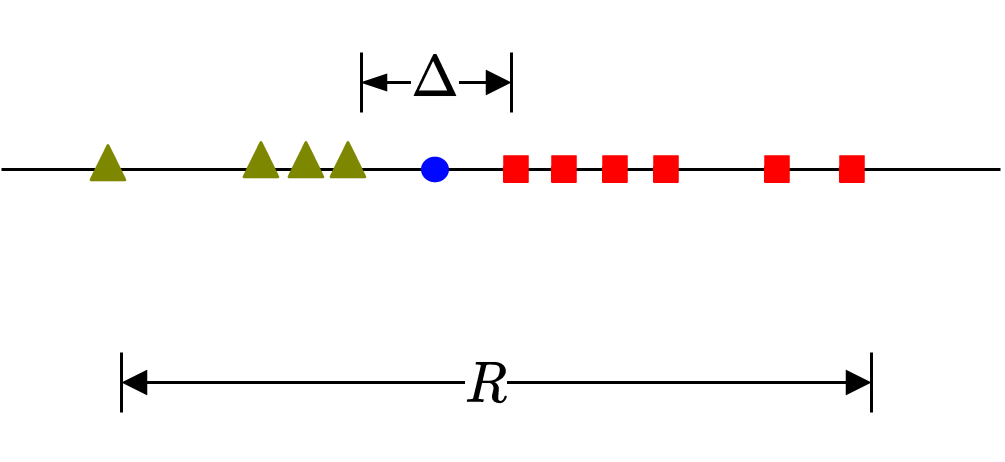
\includegraphics[width=.7\linewidth]{/home/mridul/Desktop/iitd_rishi_laptop/backups/ELL888/margin_func.png}
    \caption{\label{fig:1}Data points $\in\mathbb{R}^1$}
\end{figure}
\begin{figure}[!htbp]
    \centering
    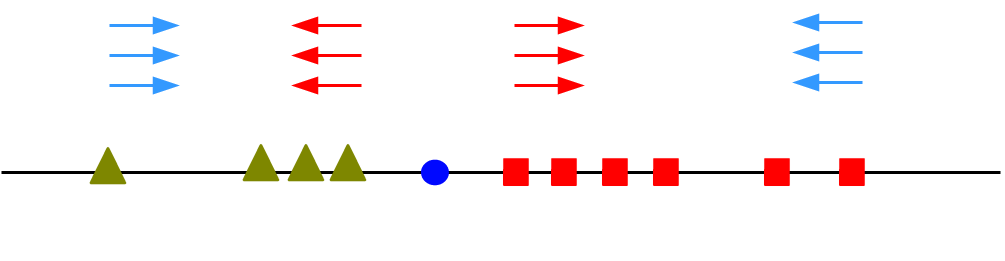
\includegraphics[width=.7\linewidth]{/home/mridul/Desktop/iitd_rishi_laptop/backups/ELL888/margin_func2.png}
    \caption{\label{fig:2}The red arrows are operations on margin and blue
    arrows on radius}
\end{figure}
\subsubsection{MCM formulations}
The mathematical formulations of MCM~\cite{MCM} start by defining a
mathematical quantity $h_{MCM}$ as
\begin{equation}
    h_{MCM}=\frac{\max_{i=1,2,\dotsc,M}\lVert u^Tx_i+v\rVert}{\min_{i=1,2,\dotsc,M}\lVert u^Tx_i+v\rVert}
\end{equation}
where it is assumed that the separating hyperplane is $u^Tx+v=0$. It is assumed
that the data are linearly separable.\par
Augmenting the data mathbftors to have a feature whose value is always 1, and
concatenating the weight mathbftor, we have $\hat{x}_i\gets\{x_i;1\}$ and
$\hat{u}\gets \{u;v\}$. Then the hyperplane goes through the origin in the
$\mathbb{R}^{(n+1)}$ space.\par
Then, the margin $\Delta$ is given by
\begin{equation}
    \Delta=\min_{i=1,2,\dotsc,M}\frac{\lVert\hat{u}^T\hat{x}_i\rVert}{\lVert\hat{u}\rVert}
\end{equation}
and the radius is just $R=\max_{i=1,2,\dotsc,M}\lVert\hat{x}_i\rVert$. So, the
ratio of interest $\dfrac{R}{\Delta}$ is given by:
\begin{equation}
    \frac{R}{\Delta}=\frac{\max_{i=1,2,\dotsc,M}\lVert\hat{x}_i\rVert}{\min_{i=1,2,\dotsc,M}\frac{\lVert\hat{u}^T\hat{x}_i\rVert}{\lVert\hat{u}\rVert}}=\frac{\max_{i=1,2,\dotsc,M}\lVert\hat{u}\rVert\lVert\hat{x}_i\rVert}{\min_{i=1,2,\dotsc,M}\lVert\hat{u}^T\hat{x}_i\rVert}
\end{equation}
And using the Cauchy-Schwarz inequality ($\lVert a^Tb\rVert\le\lVert
a\rVert\lvert b\rVert$)
\begin{equation}
    \frac{R}{\Delta}\ge\frac{\max_{i=1,2,\dotsc,M}\lVert\hat{u}^T\hat{x}_i\rVert}{\min_{i=1,2,\dotsc,M}\lVert\hat{u}^T\hat{x}_i\rVert}=\frac{\max_{i=1,2,\dotsc,M}\lVert u^Tx_i+v\rVert}{\min_{i=1,2,\dotsc,M}\lVert
    u^Tx_i+v\rVert}
\end{equation}
Thus
\begin{align}
    h_{MCM}&\le\frac{R}{\Delta}\\
    \Rightarrow
    h_{MCM}^2&\le\left(\frac{R}{\Delta}\right)^2<1+\left(\frac{R}{\Delta}\right)^2
\end{align}
From equation~\ref{eq:vcbound} we have for large dimensional data:
\begin{equation}
    h\le 1+\left(\frac{R}{\Delta}\right)^2
\end{equation}
Thus $\exists\beta\in\mathbb{R}^+,$ such that $h\le\beta h_{MCM}^2$. Also since,
$h_{MCM}^2\ge 1$ and VC-dimension satisfies $h\ge 1$,
$\exists\alpha\in\mathbb{R},\alpha>0$ such that $\alpha h_{MCM}^2\le h$.
Combining the two we have $\exists \alpha,\beta > 0, \alpha,\beta\in\mathbb{R}$
such that
\begin{equation}
    \alpha h_{MCM}^2\le h\le\beta h_{MCM}^2
\end{equation}
That is $h^2_{MCM}$ is an exact bound on the VC dimension $h$. And since the
data are linearly separable, $u^Tx_i+v\ge 0$ if $y_i=1$ and $u^Tx_i+v\le 0$ if
$y_i=-1$. Thus $\lVert u^Tx_i+v\rVert$ can be written as $y_i(u^Tx_i+v)$. Thus
the machine capacity can be minimized by keeping $h_{MCM}^2$ as small as
possible.
\begin{equation}
    \underset{u,v}{\operatorname{minimize}}\;\; h_{MCM}=\frac{\max_{i=1,\dotsc,M}y_i(u^Tx_i+v)}{\min_{i=1,\dotsc,M}y_i(u^Tx_i+v)}
\end{equation}
Further the authors show that the above formulation can be simplified
by writing:
\begin{align}
    &h_{MCM}=\frac{g}{l}\\
    &\min_{u,v,g,l}\frac{g}{l}\quad\text{subject to}\\
    &g\ge y_i(u^Tx_i+v),\quad i=1,\dotsc,M\\
    &l\le y_i(u^Tx_i+v),\quad i=1,\dotsc,M
\end{align}
Using Charnes-Cooper transformation, introducing $p=\frac{1}{l}$
\begin{align}
    &\min_{u,v,g,l,p}g\cdot p\quad\text{subject to}\\
    &g\cdot p\ge y_i(p\cdot u^Tx_i+p\cdot v),\quad i=1,\dotsc,M\\
    &l\cdot p\le y_i(p\cdot u^Tx_i+p\cdot v),\quad i=1,\dotsc,M\\
    &p\cdot l=1
\end{align}
Denoting $w\stackrel{\Delta}{=}p\cdot u,b\stackrel{\Delta}{=}p\cdot v$ and
noting that $p\cdot l=1$
\begin{align}
    &\label{eq:1}\min_{w,b,h}h\quad\text{subject to}\\
    &\label{eq:2}h\ge y_i(w^Tx_i+b),\quad i=1,\dotsc,M\\
    &\label{eq:3}1\le y_i(w^Tx_i+b),\quad i=1,\dotsc,M
\end{align}
Equations~\ref{eq:1}-\ref{eq:3} define the Minimal Complexity Machine (MCM). And
it is trained by solving the Linear Programming Problem defined above.
\subsubsection{Generalizing the MCM}
The MCM above is generalized to allow for classification errors by
introducing slack variables.
\begin{align*}
    &\min_{w,b,h,q}h+C\cdot\sum_{i=1}^Mq_i\\
    &h\ge y_i(w^Tx_i+b)+q_i,\quad i=1,\dotsc,M\\
    &1\le y_i(w^Tx_i+b)+q_i,\quad i=1,\dotsc,M\\
    &q_i\ge 0\quad i=1,\dotsc,M
\end{align*}
And for the non-linear case using Kernels
\begin{align}
    &\min_{w,b,h,q}h+C\cdot\sum_{i=1}^Mq_i\\
    &h\ge y_i(w^T\phi(x_i)+b)+q_i,\quad i=1,\dotsc,M\\
    &1\le y_i(w^T\phi(x_i)+b)+q_i,\quad i=1,\dotsc,M\\
    &q_i\ge 0\quad i=1,\dotsc,M
\end{align}
where $\phi(\cdot)$ is the mapping function that maps input to a higher
dimensional space, where the inputs are assumed to be linearly separable with
some errors. As of yet, this doesn't use a kernel function $K(\cdot,\cdot)$. Assume that $K$
is a kernel function corresponding to the map $\phi(\cdot)$;
$\phi(x_j)^T\phi(x_k)=K(x_j,x_k)$. Also, since $\phi(x_i), i=1,\dotsc,M$ forms a
basis for the feature space in which $w$ lies, $w$ can be written as a linear
combination of the basis mathbftors
\begin{align*}
    &w=\sum_{j=1}^M\lambda_j\phi(x_j)\\
    &\Rightarrow
    w^T\phi(x_i)=\sum_{j=1}^M\lambda_j\phi(x_j)^T\phi(x_i)=\sum_{j=1}^M\lambda_jK(x_j,x_i)
\end{align*}
Now, the MCM formulation can be rewritten using $K(\cdot,\cdot)$ as
\begin{align}
    &\label{eq:mcmstart}\min_{\lambda,b,h,q}h+C\cdot\sum_{i=1}^Mq_i\quad\text{subject to}\\
    &\label{eq:upbound}h\ge y_i\left(\sum_{j=1}^M\lambda_jK(x_j,x_i)+b\right)+q_i,\quad i=1,\dotsc,M\\
    &1\le y_i\left(\sum_{j=1}^M\lambda_jK(x_j,x_i)+b\right)+q_i,\quad i=1,\dotsc,M\\
    &\label{eq:mcmend}q_i\ge 0\quad i=1,\dotsc,M
\end{align}
After optimizing, those mathbftors $x_i$ for which the corresponding $\lambda_i$ is
non zero form the support mathbftors that support $w$.
$SV=\{i\;\lvert\;\lambda_i\ne 0\}$. One last
thing that needs to be defined explicitly is how to predict on new data once the
optimization is complete. The class is assigned as:
\[y_{\text{pred}}=\operatorname{sign}\left(\sum_{i\in
SV}\lambda_iK(x_i,x_{\text{test}})+b\right)\]
This completes the MCM formulation. One thing to note is Vapnik's SVM
formulation was also motivated from the fact that constraining the VC-dimension
will improve generalization, but Vapnik does this by only trying to maximize the
margin $\Delta$, whereas in MCM the ratio $R/\Delta$ is constrained to control the
complexity of the machine. This results in an extra constraint bounding the
maximum distance from the hyperplane from above (eq.~\ref{eq:upbound}), thus
providing actual theoretical guarantees. It has also been experimentally showed
that the number of support mathbftors (and thus the size itself of MCM) is much
smaller, allowing these machines to be used in edge devices where neural
networks can't be used.
\begin{figure}
    \centering
    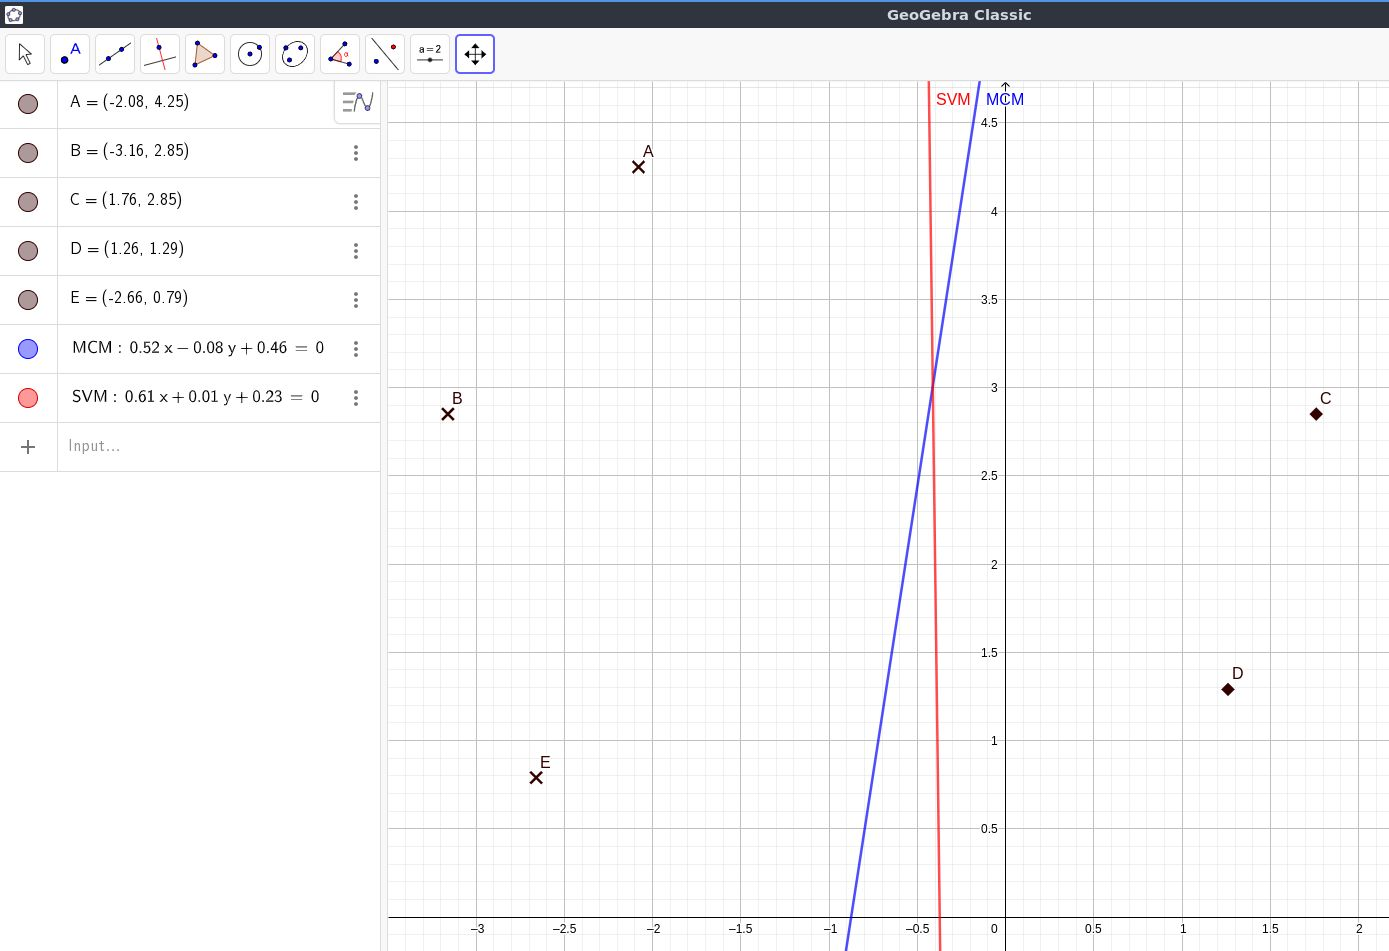
\includegraphics[draft=false,width=.8\linewidth]{/home/mridul/Desktop/iitd_rishi_laptop/backups/ELL888/MCM_vs_SVM.jpg}
    \caption{\label{fig:mcmvsvm}Separating hyperplanes learned by MCM and SVM}
\end{figure}
In figure~\ref{fig:mcmvsvm}, I take a very simple two dimensional dataset, and
solve a linear MCM without slack using an online linear programming solver. To compare with SVM, I
use \texttt{scikit-learn}'s \texttt{LinearSVC} module with a very high value of
C (so basically without slack) and plot the decision boundaries for the two.
It's not at all apparent that one of them has VC-dimension bound by a known
number as a side effect of optimization, whereas the other doesn't. And the
difference in performance on test dataset can only be understood by looking at
the numbers.\par
{\bf Note:} Since MCM is linear optimization, the kernel is not required to be
positive definite from the optimization perspective. From the SVM theory
perspective, it'll then not lie in the familiar Reproducing Kernel Hilbert
Space. It'll instead lie in a {\em Krein space} and the inner product will have
to be adjusted accordingly. We only consider Mercer Kernels.
\afterpage{\clearpage}
\subsection{Kernel Optimization}
The key ideas for kernel optimization comes from~\cite{amari}. When the data are
non-linearly separable, it is assumed that when projected to a space of high
enough dimension, they'll be separable. But this is only true when the
mapping function is suitably chosen. No kernel defeats all
others. If the kernel is ``wrong'' for the current task, the class separability
in the feature space/image space may be poorer than it was in input space.
\subsubsection{Motivation}
Again let's consider the data shown in figure~\ref{fig:1}. Even though the data
are already linearly separable, let's see what we can do to improve the class
separability. Consider figures~\ref{fig:3}-\ref{fig:5}. We can see that if we
magnify around the feature space around the class boundary (near hyperplane)
while compressing the space around the edges, we can improve class separability
thus improving generalization.
\begin{figure}[!htbp]
    \centering
    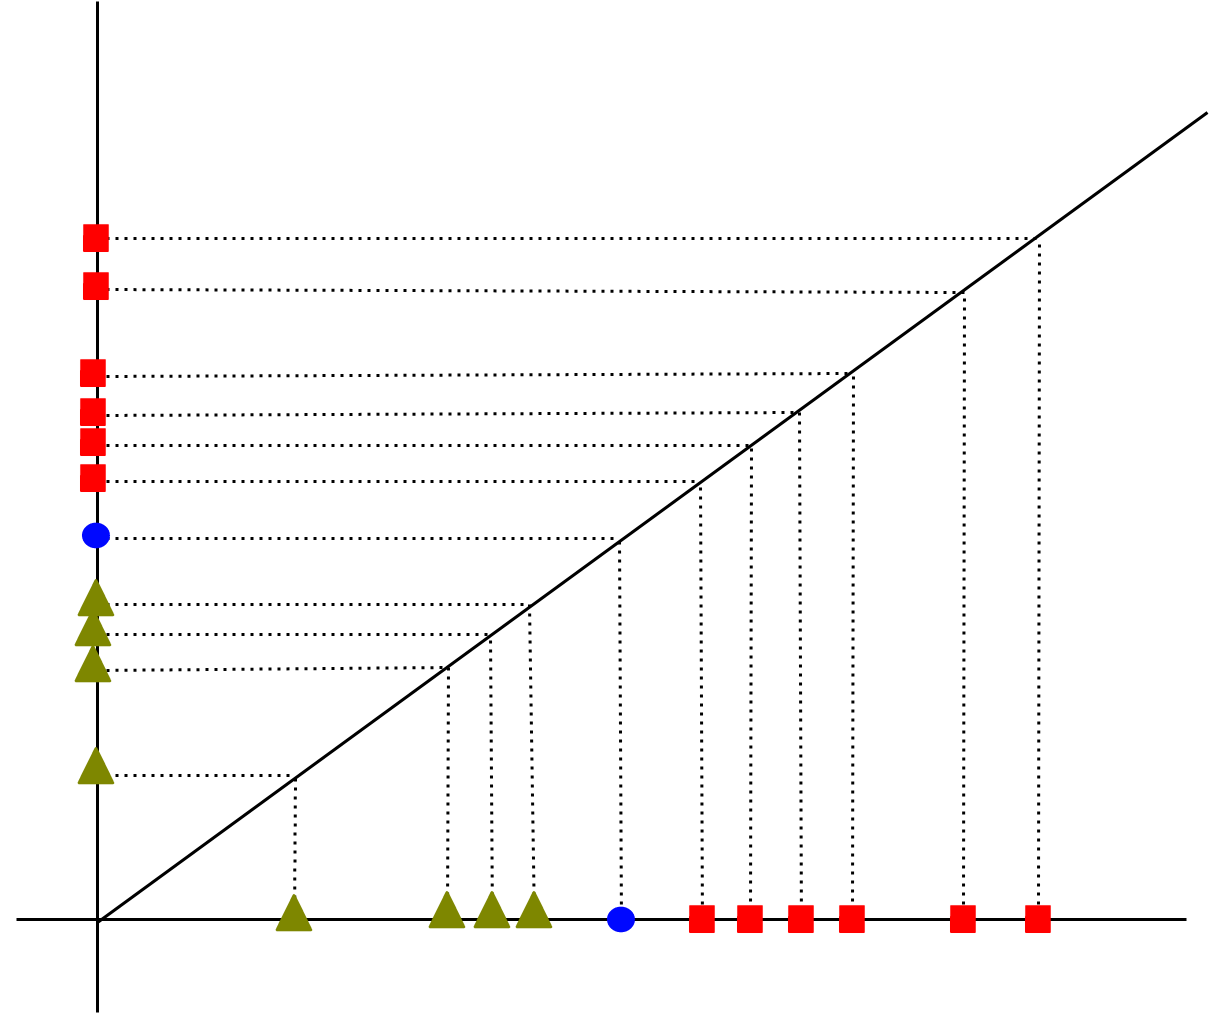
\includegraphics[width=.5\linewidth]{/home/mridul/Desktop/iitd_rishi_laptop/backups/ELL888/margin_func3.png}
    \caption{\label{fig:3}Identity map, to compare with}
\end{figure}
\begin{figure}[!htbp]
    \centering
    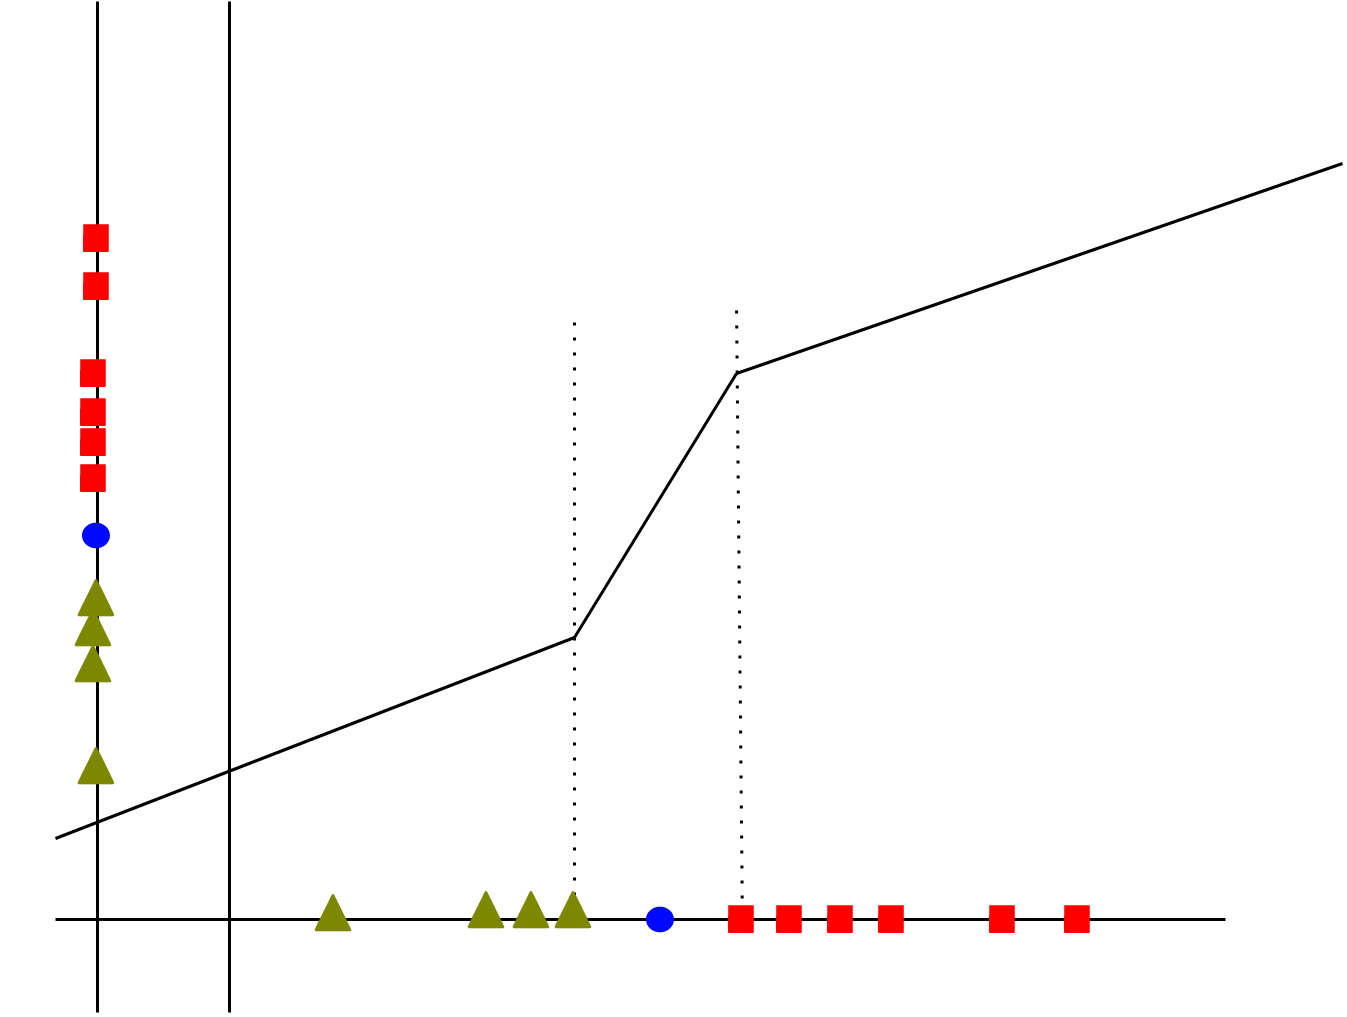
\includegraphics[width=.5\linewidth]{/home/mridul/Desktop/iitd_rishi_laptop/backups/ELL888/margin_func4.png}
    \caption{\label{fig:4}A non-linear map that is steeper between the classes,
    shallower within (data dependent)}
\end{figure}
\begin{figure}[!htbp]
    \centering
    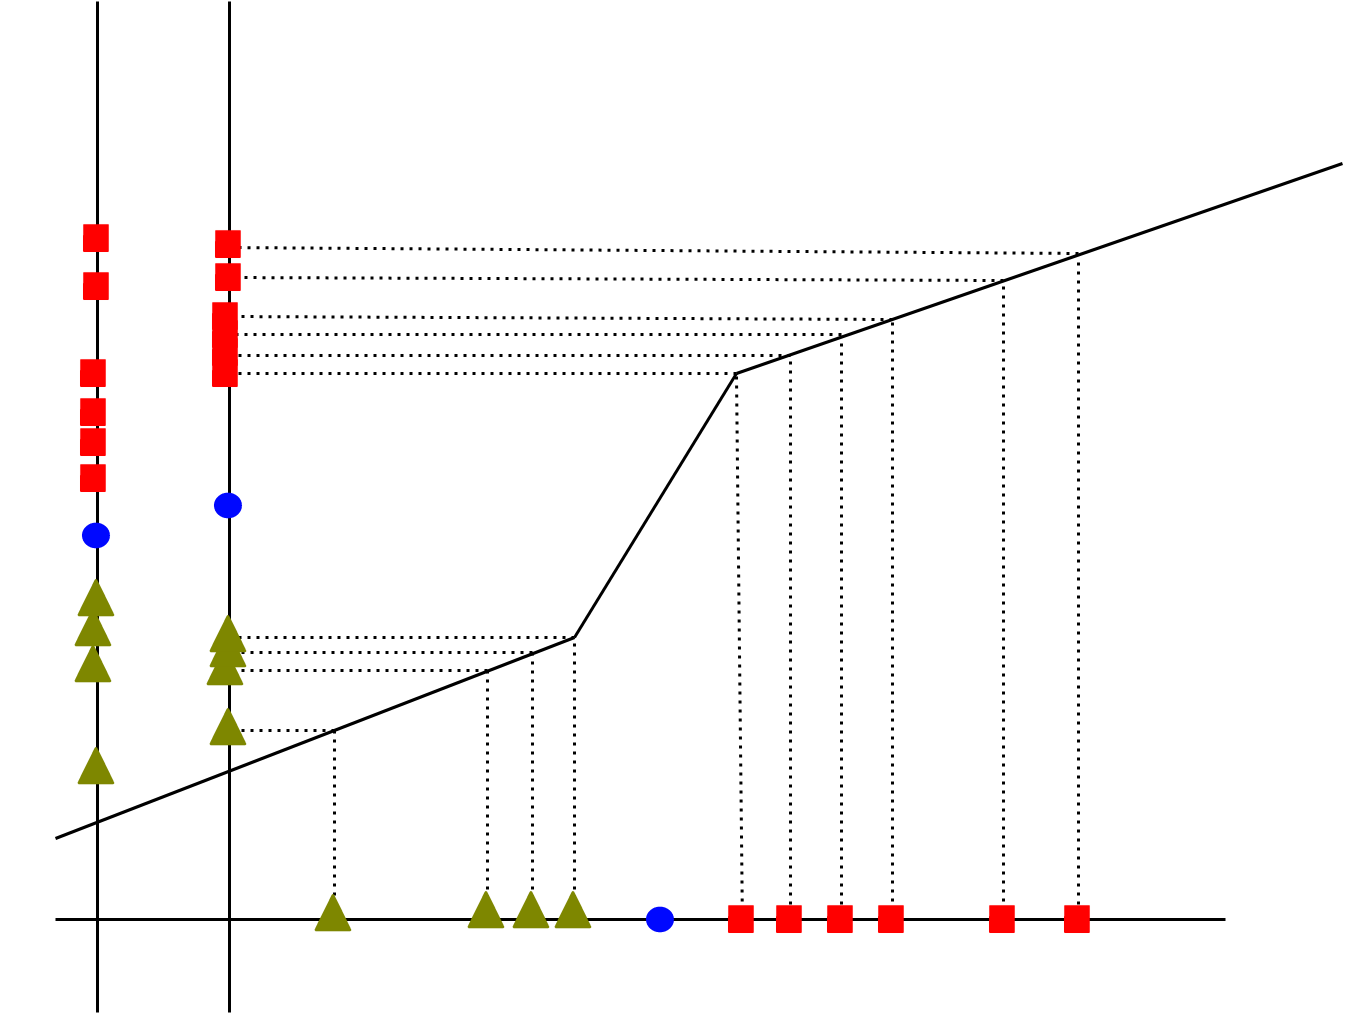
\includegraphics[width=.5\linewidth]{/home/mridul/Desktop/iitd_rishi_laptop/backups/ELL888/margin_func5.png}
    \caption{\label{fig:5}This improves class separability, and also compresses
    the data reducing VC-dimension}
\end{figure}
\subsubsection{Formulations}
This is approximately what Amari \etal\ do. They do not compress around the
edges, but just focus on magnifying on the confusion region, the boundary while
leaving the radius intact. That
is they try to increase the margin even further by having an appropriate
distortion. Since the boundary is not generally known, magnification is done
close to support mathbftors, since they are close to the boundary. These are called
``empirical cores'' in the context of kernel optimization (since after
optimization the actual support mathbftors will be different).\par
The ``magnification'' is done by applying a {\em conformal transformation} to
the kernel. Conformal transformation of a space preserves angles but may
change lengths locally, which is just what we need, to magnify without altering
angular structures. Conformal transformation of the kernel \textit{by a factor
$c(x)$} is given by:
\[\tilde{K}(x,x')=c(x)c(x')K(x,x')\]
This transformation function is constructed in a data dependent way to be
maximal around support mathbftors. For more detail about how to arrive at this, and
the underlying Riemannian metric tensor based theory, refer~\cite{amari}.\par
This work is taken further by Xiong \etal~\cite{xiong}. Until now we have been
talking about ``class separability'' subjectively, but Xiong \etal\ solidify
this by giving an actual mathematical formulation of class separability that can
be used to guide the kernel optimization. But first define the factor function
they use
\begin{align*}
    &k(x,y)=c(x)c(y)k_0(x,y)\\
    &c(x)=\alpha_0+\sum_{i=1}^{n_{ec}}\alpha_ik_1(x,a_i)
\end{align*}
$k_0(\cdot,\cdot)$ is a basic kernel, like Gaussian.
$k_1(x,a_i)=\exp(-\gamma\lVert x-a_i\rVert^2)$ and $a_i$ are ``empirical
cores''. We can see that $k_1(x,a_i)$ is maximum near $a_i$, and thus most
magnification is around the empirical cores. Also, to get an intuitive sense of
``magnification'', consider that the $k_0(\cdot,\cdot)$ is some sort of distance
or similarity measure (that's what the Riemannian metric implies, measure of
distances). $\alpha_i$'s are called combination coefficients. It is easy to write
the matrix notation of these by defining $K\text{ and }K_0$ as the matrix
corresponding to $k(\cdot,\cdot)$ and $k_0(\cdot,\cdot)$ respectively.
\[K=[c(x_i)c(x_j)k_0(x_i,x_j)]_{M\times M}=CK_0C\]
where $C=diag(c(x_1),c(x_2),\dotsc,c(x_M))$. Furthermore
\begin{equation}
    \label{eq:alk}
    \mathbf{c}=\begin{pmatrix}
        1&k_1(x_1,a_1)&\dots&k_1(x_1,a_{n_{ec}})\\
        1&k_2(x_2,a_1)&\dots&k_1(x_2,a_{n_{ec}})\\
        \vdots&\vdots&\ddots&\vdots\\
        1&k_M(x_M,a_1)&\dots&k_1(x_M,a_{n_{ec}})\\
        \end{pmatrix}\begin{pmatrix}
            \alpha_0\\
            \alpha_1\\
            \vdots\\
            \alpha_{n_{ec}}
    \end{pmatrix}\stackrel{\Delta}{=}K_1\mathbf{\alpha}
\end{equation}
where $K_1$ is an $M\times(n_{ec}+1)$ matrix.\par
Next, they use a measure of class separability called {\em Fisher scalar} to
define their own Kernel based class separability metric. The Fisher scalar is
defined as
\begin{align}
    &J=\frac{\operatorname{tr} S_b}{\operatorname{tr} S_w}\\
    &S_b=\frac{1}{M}\sum_{i=1}^2M_i(\bar{z}_i-\bar{z})(\bar{z}_i-\bar{z})^T\\
    &S_w=\frac{1}{M}\sum_{i=1}^2\sum_{j=1}^{M_i}(z_j^i-\bar{z}_i)(z_j^i-\bar{z}_i)^T
\end{align}
where $i$ indexes through the two classes, $M_i$ is the number of samples in the
$i^\text{th}$ class. $\{z_j\}_{j=1}^M$ are the images of the training data in
the empirical feature space. $M_1+M_2=M$. $\bar{z},\bar{z}_1,\bar{z}_2$ are the
centers of the entire training data and those of class 1 and 2 resepctively in
the empirical feature space. $z_j^i$ is the $j^\text{th}$ data sample in
$i^\text{th}$ class. $S_b$ and $S_w$ are the between-class scatter and
within-class scatter. Reducing the within-class scatter reduces the neighborhood
size, thus reducing the radius. While increasing the between-class scatter
increases the distances between the samples of different classes. Thus the
chances of misclassification in a dense neighborhood go down (or structural risk
goes down). This is why we want maximize $J$.
\begin{figure}[!htbp]
    \centering
    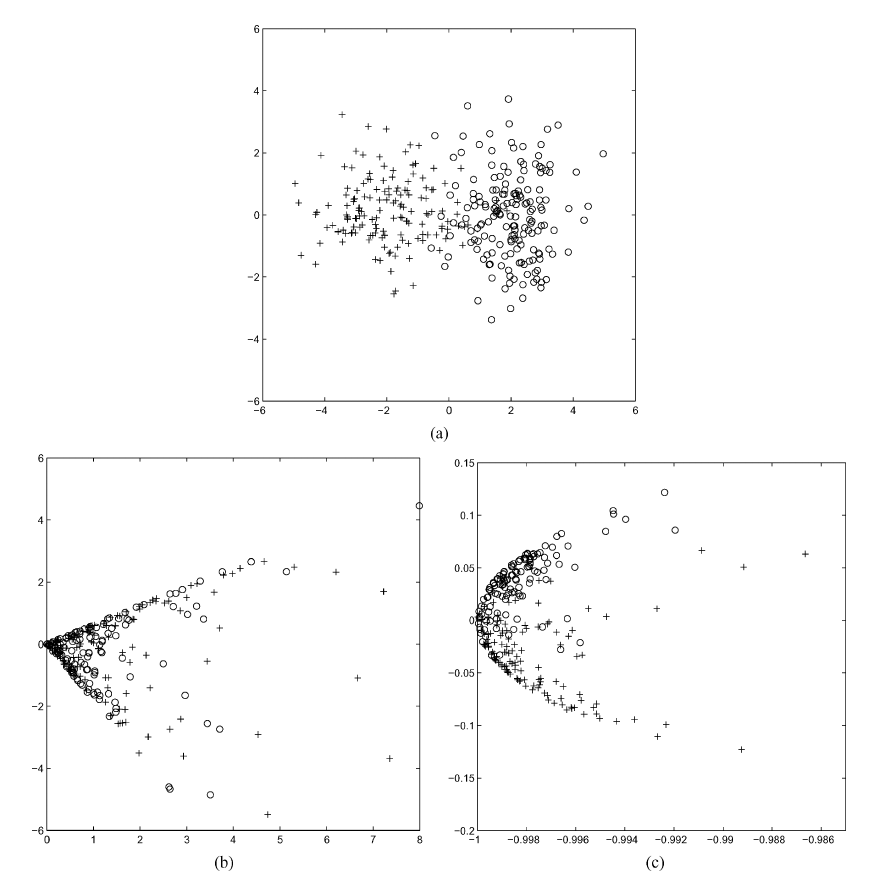
\includegraphics[width=.8\linewidth]{/home/mridul/Desktop/iitd_rishi_laptop/backups/ELL888/class_sep.png}
    \caption{\label{fig:6}This picture is taken from Xiong {\em et
    al.}~\cite{xiong}.  It shows how a kernel can harm class separability. (a)
    Input. (b) Two dimensional projection of empirical feature space for second
    order polynomial kernel. (c) Two dimensional projection of Gaussian kernel.}
\end{figure}
\par
This can be further simplified by ordering the data points such that the first
$M_1$ points belong to class 1, $y_i=-1,i\le M_1$ and the remaining belong to
class 2. Then kernel matrix can be written in a block form as:
\[K=\begin{pmatrix}K_{11}&K_{12}\\K_{21}&K_{22}\end{pmatrix}\]
$K_{11}$ is an $M_1\times M_1$ submatrix of $K$ that corresponds to class 1.
Similarly $K_{22}$ is an $M_2\times M_2$ sized matrix corresponding to class 2.
$K_{12}\text{ and }K_{21}$ are $M_1\times M_2\text{ and }M_2\times M_1$
respectively. Next define ``between-class'' and ``within-class'' kernel scatter
matrices $B\text{ and }W$ as:
\begin{align}
    \label{eq:B}B=&\begin{pmatrix}
        \frac{1}{M_1}K_{11}&0\\
        0&\frac{1}{M_2}K_{22}
        \end{pmatrix}-\begin{pmatrix}
            \frac{1}{M}K_{11}&\frac{1}{M}K_{12}\\
            \frac{1}{M}K_{21}&\frac{1}{M}K_{22}
    \end{pmatrix}\\
    \label{eq:W}W=&\begin{pmatrix}
        k_{11} & 0 & \dots & 0\\
        0 & k_{22} & \dots & 0\\
        \vdots & \vdots & \ddots & \vdots\\
        0 & 0 & \dots & k_{MM}
        \end{pmatrix}-\begin{pmatrix}\frac{1}{M_1}K_{11}&0\\0&\frac{1}{M_2}K_{22}\end{pmatrix}
\end{align}
Also, denote $B_0$ and $W_0$ as the between-class and within-class kernel
scatter matrices corresponding to the basic kernel $K_0$.
{\theorem (Xiong \etal) Let $1_k$ be the $k$-dimensional mathbftor whose
entries are all equal to one. Then
\begin{equation}
    \label{eq:gep}
    J=\frac{1_M^TB1_M}{1_M^TW1_M}=\frac{\mathbf{c}^TB_0\mathbf{c}}{\mathbf{c}^TW_0\mathbf{c}}
\end{equation}
Proof: refer~\cite{xiong}
}
Xiong \etal\ then optimize the kernel such that the class separability metric $J$
is maximized using a gradient based approach. Here we diverge to the approach
used by Jayadeva \etal\ in~\cite{keropt}. Instead of solving as a gradient based
optimization, they identify the Rayleigh Quotient in equation~\ref{eq:gep} and
naturally propose it as a Generalized Eigenvalue Problem and try to solve
simultaneously for $\gamma$ and $\mathbf{c}$ in
\[B_0\mathbf{c}=\gamma W_0\mathbf{c}
\]
where $\gamma$ is the set of eigenvalues. This is further rewritten using
equation~\ref{eq:alk} as $[K_1^TB_0K_1]\mathbf{\alpha}=\gamma[K_1^T(W_0+DI)K_1]\mathbf{\alpha}$.
$D$ is a small constant added to the diagonal values for stability, $I$ is
identity matrix. Let $K_1^TB_0K_1\stackrel{\Delta}{=}P,
[K_1^T(W_0+DI)K_1]\stackrel{\Delta}{=}Q$. So we have 
\begin{equation}
    \label{eq:GEP}P\mathbf{\alpha}=\gamma Q\mathbf{\alpha}
\end{equation}\par
From the solution we can get $\mathbf{\alpha}$ (corresponding to maximum eigenvalue
$\gamma$), which in turn gives $\mathbf{c}$, which in turn gives the conformal
map transformed kernel $K$. And, finally we have enough theory to discuss Kernel
optimization for MCMs. Note, all the previous theory regarding kernel
optimization was in context of support mathbftor machines (SVMs).
\section{Kernel optimization using conformal maps for the minimal complexity
machine~\cite{keropt}}
We have basically every ingredient necessary to talk about this: we have the
motivation to use MCMs, we have the motivation and the method to perform
kernel optimization, we have the statistical learning theory backing up our
intuition that separating out classes should improve generalization. Now let's talk about how
kernel optimization is done in the context of MCMs. It's just a simple
algorithm:
\begin{enumerate}
    \item Transform the dataset to zero mean and unit variance.
    \item Solve the optimization defined in
        equations~\ref{eq:mcmstart}-\ref{eq:mcmend} using the basic kernel to
        get support mathbftors for which $\lambda_i \ne 0$ (or to account for
        computational limitations, $\lvert\lambda_i\rvert > \varepsilon$ where
        $\varepsilon$ is a small constant.
    \item Compute $W_0$, $B_0$ (eq~\ref{eq:W},\ref{eq:B})
    \item Solve the generalized eigenvalue problem in equation~\ref{eq:GEP} to
        find $\mathbf{\alpha}$ corresponding to largest eigen value.
    \item Use $\mathbf{\alpha}$ to compute the scaling factor $\mathbf{c}$
    \item Use the scaling factor to compute the optimized kernel
        $k(x_i,x_j)=c(x_i)c(x_j)k_0(x_i,x_j)$
    \item Use the optimized kernel matrix $K(\cdot,\cdot)$ corresponding to
        kernel function $k(\cdot,\cdot)$ to train a new MCM (that is again solve
        equations~\ref{eq:mcmstart}-\ref{eq:mcmend}.)
    \item Use this new MCM on test data.
\end{enumerate}
\par
Results in~\cite{keropt} shows that MCM with optimized kernels perform better when
measured by accuracy by a big margin for almost all of the benchmark datasets as
compared with vanilla MCM or SVM.  The maximum number of samples in any of these
datasets was 1000. When applied on datasets of larger size, the MCM's do not
perform much better, which is expected from equation~\ref{eq:vareps}. As $M$,
the training sample size plays a much larger role in reducing $\varepsilon$ and
in turn reducing the structural risk, it doesn't help a lot in big data setting
to focus on structural risk minimization. But MCMs still provide a sparser model
to be deployed on power constrained devices.
\afterpage{\clearpage}


	
	\bibliographystyle{plain}
	\begin{thebibliography}{10}
        \bibitem{amari}
            Amari SI, Wu S. 
            \newblock{\em Improving support mathbftor machine classifiers by modifying kernel functions.}.
            \newblock Neural Networks. 1999 Jul 1;12(6):783-9.
        \bibitem{slt}
            Vapnik VN. 
            \newblock{\em An overview of statistical learning theory.}
            \newblock IEEE transactions on neural networks. 1999 Sep;10(5):988-99.
        \bibitem{MCM}
            Jayadeva. \newblock{\em Learning a hyperplane classifier by minimizing an exact
            bound on the VC dimension.} \newblock Neurocomputing. 2015 Feb 3;149:683-9.
        \bibitem{xiong}
            Xiong H, Swamy MN, Ahmad MO. \newblock{\em Optimizing the kernel in the empirical
            feature space.}\newblock IEEE transactions on neural networks. 2005 Mar
            7;16(2):460-74.
        \bibitem{keropt}
            Badge S, Soman S, Chandra S, Jayadeva. \newblock{\em Kernel optimization using conformal
            maps for the minimal complexity machine.}\newblock Engineering Applications of
            Artificial Intelligence. 2021 Nov 1;106:104493.
	\end{thebibliography}
	
	
	
\end{document}
